%----------------------------------------------------------------------------
\chapter{Korábbi megoldás rövid bemutatása} \label{chapter3}
%----------------------------------------------------------------------------

A jelenlegi dolgozatom alaptémáját a 2 évvel ezelőtti licensz dolgozatom adta, miszerint az egyetemen zajló jelenlétkezelési mechanizmust szeretnénk korszerűsíteni. Korábbi megoldásom QR kód alapú megoldás volt, ami csupán egy okostelefon meglétét igényelte.
A Diák alkalmazás a Tanár alkalmazással egy QR kód segítségével kommunikált, ezáltal tudta azonosítani magát a diák az egyetemi órákon. Mindkét alkalmazásnak hozzáférése volt egy közös Firebase adatbázishoz, ahol az adatok beírásra, majd lekérdezésre kerültek.

A megvalósított rendszernek két kulcsfunkcionalitása volt:

\subparagraph* {Az azonosítóként szolgáló QR kód generálása}\
\newline

A diák alkalmazás esetén generálásra került egy QR kód, ami azonosítóként szolgált. Az azonosító tartalmazta a diák szakját, a nevét, a Neptun azonosítóját, és a biztonság növelése érdekében egy egyedi eszközazonosítót is.
Mivel az előzőleges regisztráció során a diák személyes adatai bekerültek az adatbázisba, csupán lekértük ezeket az adatokat a QR kód generálásához.


\subparagraph* {QR kód szkennelése a jelenlét rögzítéséhez}\
\newline

A diák azonosítására szolgáló QR kód értelmezése a Tanár alkalmazás segítségével történt. Ezen folyamat eredménye, hogy az adott diák jelenléti adati bekerülnek az adatbázisba, amely által igazolva lesz jelenléte az aktuális órán. 
Maga a szkennelés egy gombnyomásra történik, amely által megnyílik a kamera, és a QR kód fölé tartva feldolgozza az abba kódolt adatokat.
Az azonosítás mellett az tanár alkalmazás lehetővé tette a korábbi jelenlétek megtekintését, de ugyanakkor lehetőséget adott a jelenlétek kimentésére is különböző formátumokba, amit a Google Apps script biztosított. A mobilalkalmazáson keresztült került meghívásra az említett szkript, ami lehetővé tette a jelenlétek kimentését táblázat formájában a felhasználó által kiválasztott formátumban.

A kivitelezett megoldás jobb szemléltetése érdekében az alábbi ábrán látható a rendszer architektúrája:


\begin{figure}
	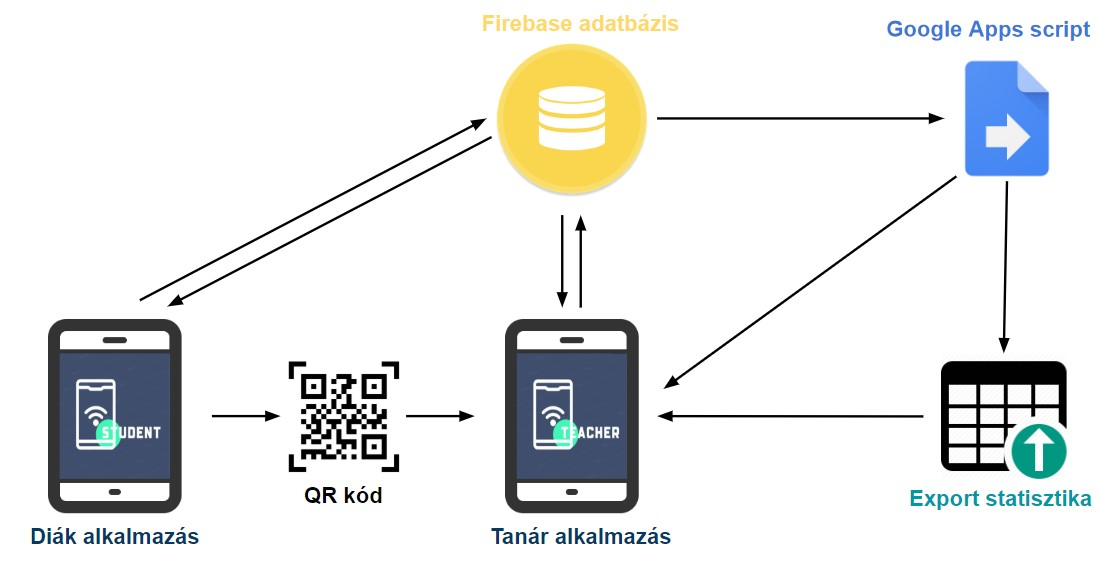
\includegraphics[width=\textwidth]{figures/architecture2.jpg}
	\caption{Az előző rendszer architektúrája}
\end{figure}

\newpage


Amint azt említettem a hallgató azonosítására szolgáló QR kód létrehozása a Diák alkalmazás feladata volt. Emellett szükséges volt egy regisztrációra és belépésre az alkalmazás funkcionalitásának igénybevételéhez, ezt követően jött létre az azonosító, illetve vissza lehetett nézni a korábbi jelenléteket. Kiegészítő funkciók közül az e-mail küldés, Neptunba és Classroom-ba való belépés volt elérhető. Mindezeket a ~\ref{fig:stud1} ábra szemlélteti.

A Tanár alkalmazáson belül elérhetőek voltak a következő funkcionalitások: regisztráció és bejelentkezés, új jelenlétek hozzáadása, korábbi jelenlétek megtekintése, jelenlétek exportálása, illetve ugyanúgy az e-mail küldési lehetőség, naptáresemény létrehozása, valamint a Google Classroom-ba történő belépés.

A Tanár applikáció három legfontosabb funkcionalitása került megjelenítésre a ~\ref{fig:teach1} ábrán.



\begin{figure}
	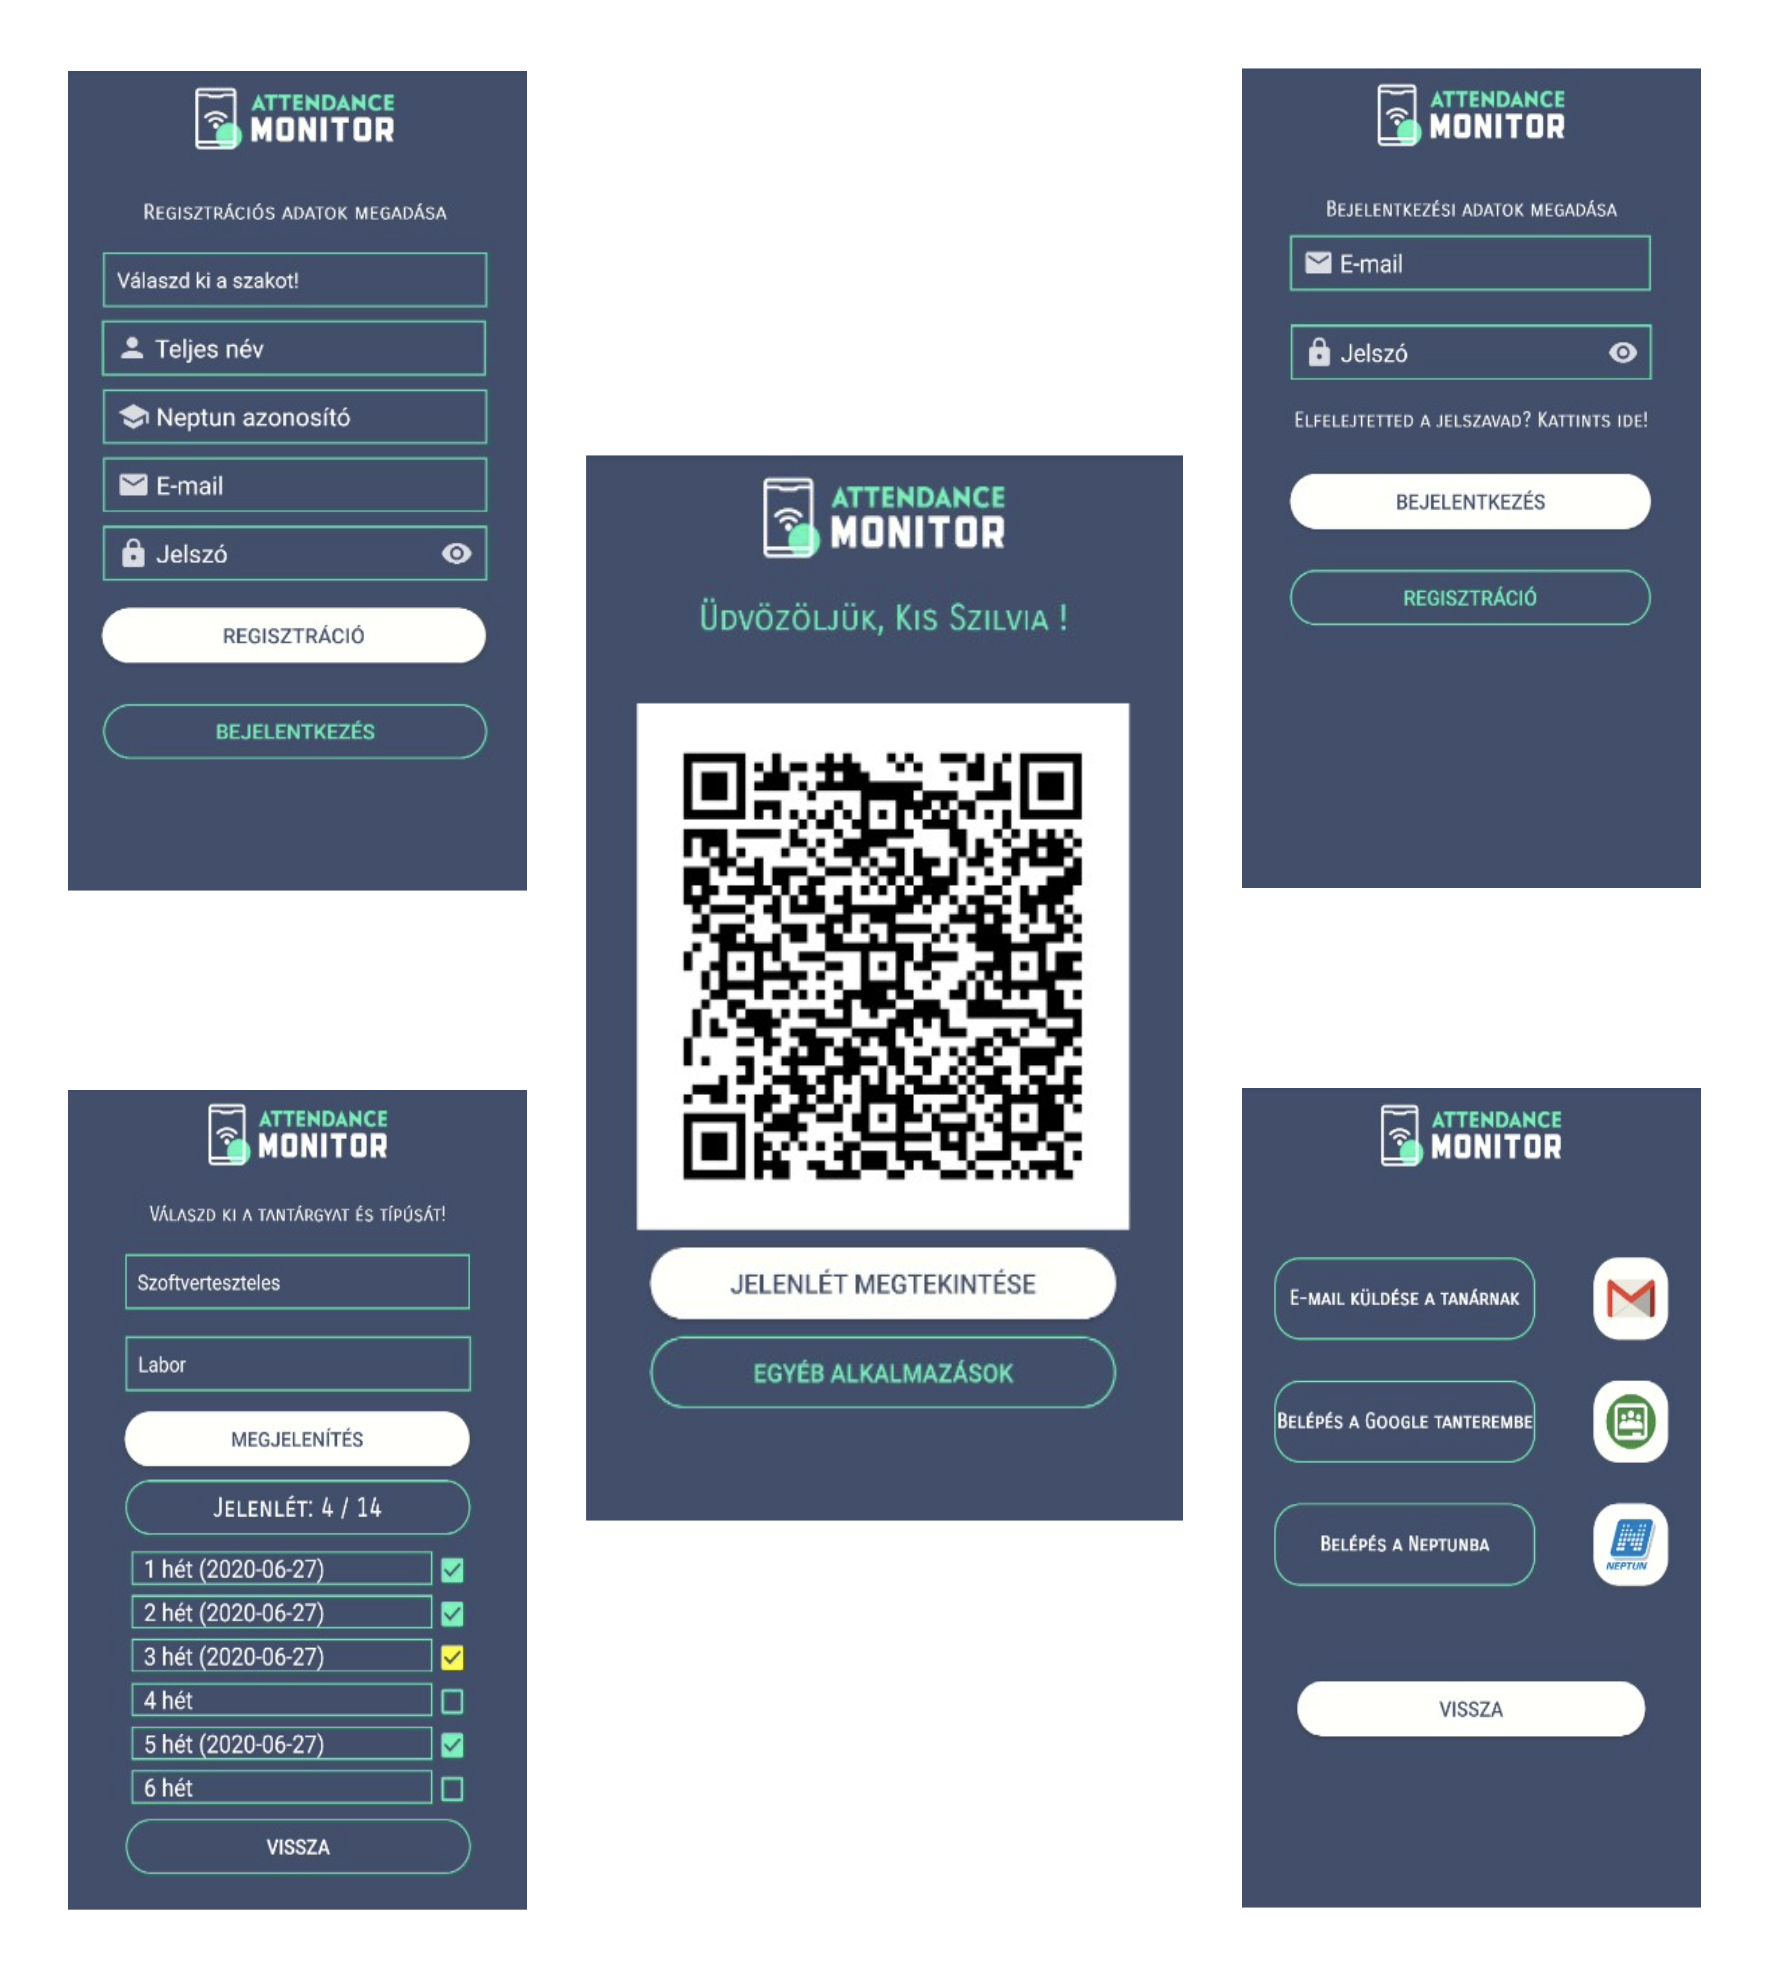
\includegraphics[width=\textwidth]{figures/stud1.png}
	\caption{Diák alkalmazás funkcionalitásai}
	\label{fig:stud1}
\end{figure}

\begin{figure}
	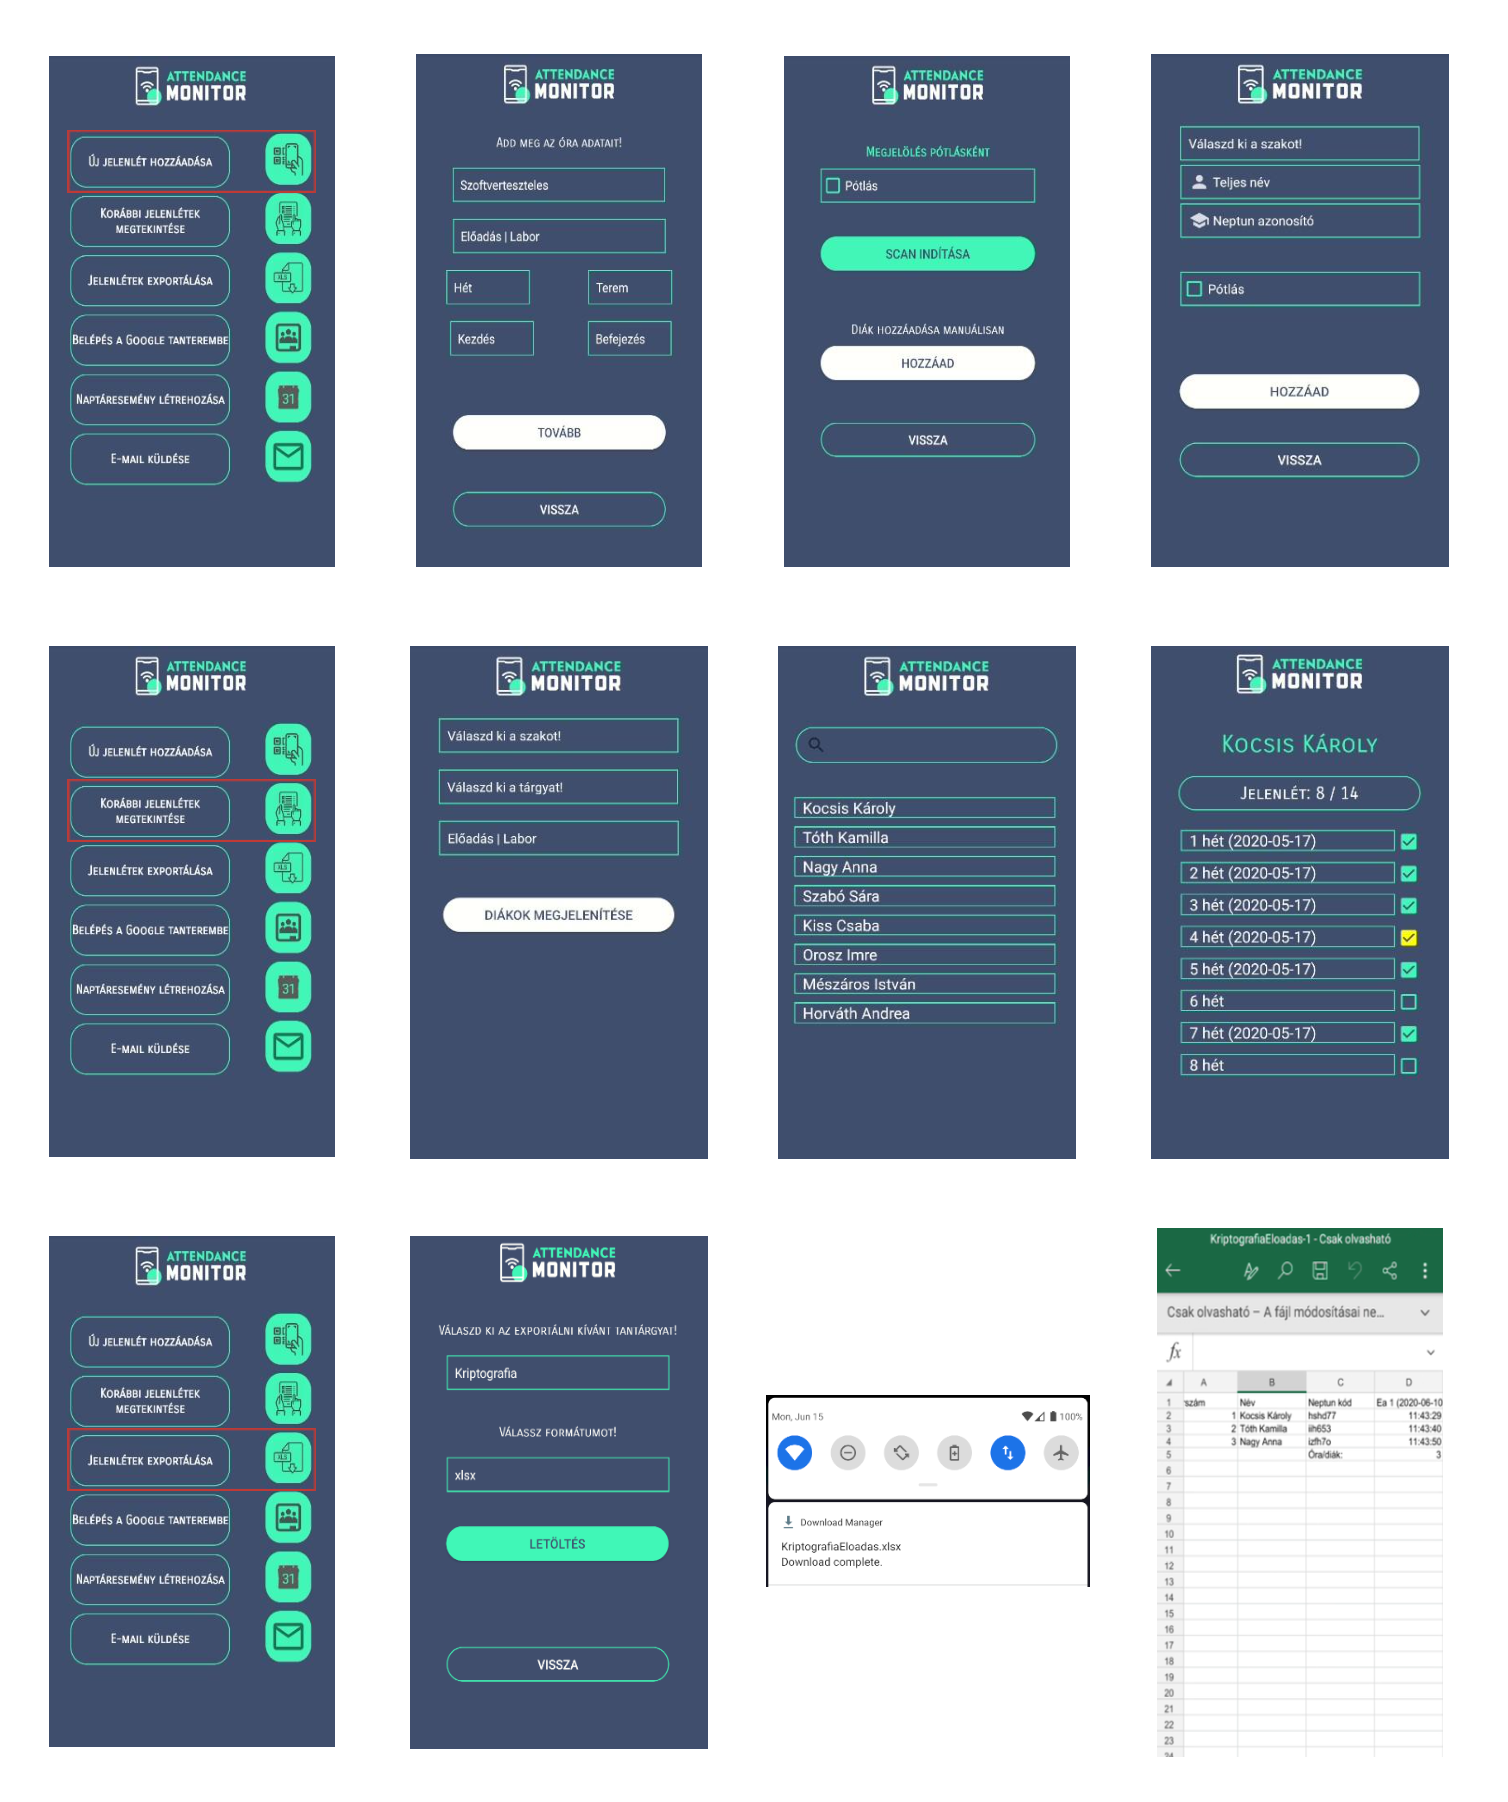
\includegraphics[width=\textwidth]{figures/teach1.png}
	\caption{Tanár alkalmazás funkcionalitásai}
	\label{fig:teach1}
\end{figure}